\documentclass[tikz,border=10pt]{standalone}
\usepackage{amsmath,amssymb}
\usepackage[scaled=0.92]{helvet}
\renewcommand{\familydefault}{\sfdefault}
\usepackage{xcolor}
\usetikzlibrary{arrows.meta,positioning,fit,backgrounds,calc,shapes.geometric,shapes.misc,patterns}

% Publication Systems Color Palette (OSDI/SOSP Style)
\definecolor{nodecteal}{HTML}{0D9488}    % Edge Ingress Tier (Node C)
\definecolor{nodecbg}{HTML}{F0FDFA}
\definecolor{nodecheader}{HTML}{0F766E}

\definecolor{nodebblue}{HTML}{2563EB}    % Regional Neural Gateway (Node B)
\definecolor{nodebbg}{HTML}{EFF6FF}
\definecolor{nodebheader}{HTML}{1D4ED8}

\definecolor{nodeaamber}{HTML}{D97706}   % Cloud Host Tier (Node A)
\definecolor{nodeabg}{HTML}{FFFBEB}
\definecolor{nodeaheader}{HTML}{B45309}

\definecolor{subboxborder}{HTML}{CBD5E1}
\definecolor{subboxbg}{HTML}{FFFFFF}

\definecolor{specgreen}{HTML}{059669}    % Speculative hint & commit
\definecolor{specgreenbg}{HTML}{ECFDF5}
\definecolor{fusedblue}{HTML}{2563EB}    % Dense & fused ranking
\definecolor{fusedbluebg}{HTML}{EFF6FF}
\definecolor{retorange}{HTML}{EA580C}    % Token stream egress
\definecolor{retorangebg}{HTML}{FFF7ED}

\definecolor{textdark}{HTML}{0F172A}
\definecolor{textmuted}{HTML}{64748B}

\begin{document}
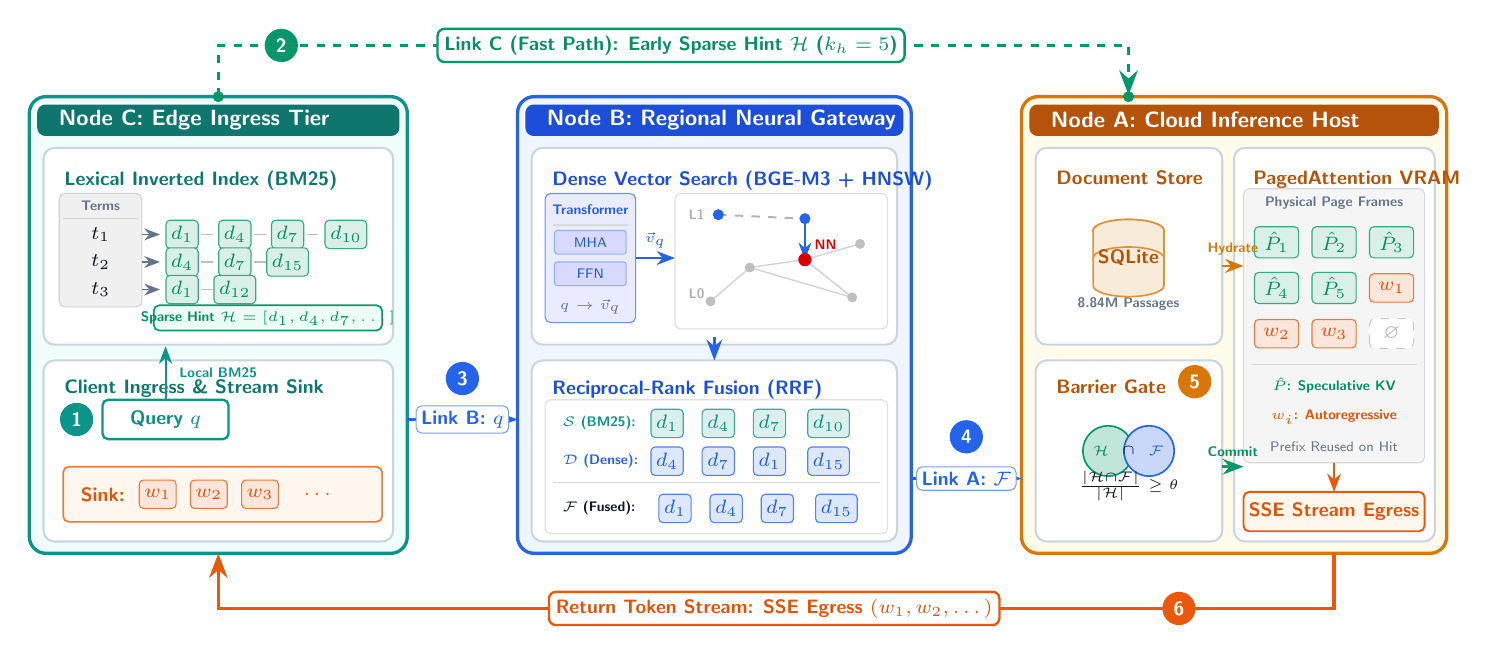
\begin{tikzpicture}[
    font=\small,
    >=Stealth,
    x=1.0cm, y=1.0cm,
    tierchassis/.style n args={2}{
        draw=#1,
        fill=#2,
        rounded corners=6pt,
        line width=1.2pt
    },
    submodule/.style={
        draw=subboxborder,
        fill=subboxbg,
        rounded corners=4pt,
        line width=0.75pt
    },
    stepnum/.style={
        circle,
        fill=#1,
        text=white,
        font=\scriptsize\bfseries,
        inner sep=0.5pt,
        minimum size=12pt
    },
    docbadge/.style={
        draw=#1!80,
        fill=#1!15,
        rounded corners=1.5pt,
        font=\scriptsize\bfseries,
        text=#1!95!black,
        inner sep=1.8pt,
        minimum height=0.36cm
    }
]

% ===========================================================================
% 1. NODE C: EDGE INGRESS TIER (x: 0.0 to 4.8, y: 0.0 to 5.8)
% ===========================================================================
\draw[tierchassis={nodecteal}{nodecbg}] (0.0, 0.0) rectangle (4.8, 5.8);
\fill[fill=nodecheader, rounded corners=3pt] (0.1, 5.30) rectangle (4.7, 5.70);
\node[anchor=west, text=white, font=\footnotesize\bfseries] at (0.25, 5.50) {Node C: Edge Ingress Tier};

% Top Submodule: Lexical Inverted Index (y: 2.65 to 5.15)
\draw[submodule] (0.18, 2.65) rectangle (4.62, 5.15);
\node[anchor=north west, font=\scriptsize\bfseries, text=nodecheader] at (0.32, 4.98) {Lexical Inverted Index (BM25)};

% Visual Inverted Index: Term Dictionary & Postings
\begin{scope}[shift={(0.38, 2.75)}]
    % Term Dict
    \draw[fill=gray!12, draw=gray!35, rounded corners=2pt] (0, 0.38) rectangle (1.05, 1.82);
    \node[font=\tiny\bfseries, text=textmuted] at (0.525, 1.66) {Terms};
    \draw[gray!35] (0.05, 1.50) -- (1.0, 1.50);
    \node[font=\scriptsize\bfseries, text=textdark] at (0.525, 1.30) {$t_1$};
    \node[font=\scriptsize\bfseries, text=textdark] at (0.525, 0.95) {$t_2$};
    \node[font=\scriptsize\bfseries, text=textdark] at (0.525, 0.60) {$t_3$};

    % Postings Pointers
    \draw[->, line width=0.6pt, draw=textmuted] (1.05, 1.30) -- (1.28, 1.30);
    \node[docbadge={specgreen}] at (1.56, 1.30) {$d_1$};
    \draw[line width=0.4pt, gray!50] (1.80, 1.30) -- (1.95, 1.30);
    \node[docbadge={specgreen}] at (2.23, 1.30) {$d_4$};
    \draw[line width=0.4pt, gray!50] (2.47, 1.30) -- (2.62, 1.30);
    \node[docbadge={specgreen}] at (2.90, 1.30) {$d_7$};
    \draw[line width=0.4pt, gray!50] (3.14, 1.30) -- (3.29, 1.30);
    \node[docbadge={specgreen}] at (3.64, 1.30) {$d_{10}$};

    \draw[->, line width=0.6pt, draw=textmuted] (1.05, 0.95) -- (1.28, 0.95);
    \node[docbadge={specgreen}] at (1.56, 0.95) {$d_4$};
    \draw[line width=0.4pt, gray!50] (1.80, 0.95) -- (1.95, 0.95);
    \node[docbadge={specgreen}] at (2.23, 0.95) {$d_7$};
    \draw[line width=0.4pt, gray!50] (2.47, 0.95) -- (2.62, 0.95);
    \node[docbadge={specgreen}] at (2.90, 0.95) {$d_{15}$};

    \draw[->, line width=0.6pt, draw=textmuted] (1.05, 0.60) -- (1.28, 0.60);
    \node[docbadge={specgreen}] at (1.56, 0.60) {$d_1$};
    \draw[line width=0.4pt, gray!50] (1.80, 0.60) -- (1.95, 0.60);
    \node[docbadge={specgreen}] at (2.23, 0.60) {$d_{12}$};

    % Early Hint Register Output
    \draw[draw=specgreen, fill=specgreenbg, rounded corners=2pt, line width=0.6pt] 
        (1.20, 0.08) rectangle (4.10, 0.40);
    \node[font=\tiny\bfseries, text=specgreen!95!black] at (2.65, 0.24) {Sparse Hint $\mathcal{H} = [d_1, d_4, d_7, \dots]$};
\end{scope}

% Bottom Submodule: Client Ingress & SSE Stream Sink (y: 0.15 to 2.45)
\draw[submodule] (0.18, 0.15) rectangle (4.62, 2.45);
\node[anchor=north west, font=\scriptsize\bfseries, text=nodecheader] at (0.32, 2.32) {Client Ingress \& Stream Sink};

\begin{scope}[shift={(0.38, 0.25)}]
    % Step 1: User Request
    \node[stepnum={nodecteal}] at (0.22, 1.45) {1};
    \draw[fill=white, draw=nodecteal, rounded corners=2pt, line width=0.85pt] (0.55, 1.20) rectangle (2.15, 1.70);
    \node[font=\scriptsize\bfseries, text=nodecteal!95!black] at (1.35, 1.45) {Query $q$};

    % Internal Dispatch to Local BM25
    \draw[->, line width=0.75pt, draw=nodecteal] (1.35, 1.70) -- (1.35, 2.38);
    \node[font=\tiny\bfseries, text=nodecteal, anchor=west] at (1.40, 2.05) {Local BM25};

    % Client Token Sink (SSE)
    \draw[fill=retorangebg, draw=retorange!80, rounded corners=2pt, line width=0.6pt] (0.05, 0.15) rectangle (4.1, 0.85);
    \node[anchor=west, font=\scriptsize\bfseries, text=retorange!95!black] at (0.15, 0.50) {Sink:};
    \node[docbadge={retorange}] at (1.25, 0.50) {$w_1$};
    \node[docbadge={retorange}] at (1.90, 0.50) {$w_2$};
    \node[docbadge={retorange}] at (2.55, 0.50) {$w_3$};
    \node[font=\scriptsize\bfseries, text=retorange] at (3.30, 0.50) {$\dots$};
\end{scope}

% ===========================================================================
% 2. NODE B: REGIONAL NEURAL GATEWAY (x: 6.2 to 11.2, y: 0.0 to 5.8)
% ===========================================================================
\draw[tierchassis={nodebblue}{nodebbg}] (6.2, 0.0) rectangle (11.2, 5.8);
\fill[fill=nodebheader, rounded corners=3pt] (6.3, 5.30) rectangle (11.1, 5.70);
\node[anchor=west, text=white, font=\footnotesize\bfseries] at (6.45, 5.50) {Node B: Regional Neural Gateway};

% Top Submodule: Dense Semantic Vector Search (y: 2.65 to 5.15)
\draw[submodule] (6.38, 2.65) rectangle (11.02, 5.15);
\node[anchor=north west, font=\scriptsize\bfseries, text=nodebheader] at (6.52, 4.98) {Dense Vector Search (BGE-M3 + HNSW)};

\begin{scope}[shift={(6.55, 2.75)}]
    % Transformer Encoder Box
    \draw[fill=blue!8, draw=nodebblue!70, rounded corners=2pt] (0.0, 0.18) rectangle (1.15, 1.82);
    \node[font=\tiny\bfseries, text=nodebblue!95!black, align=center] at (0.575, 1.62) {Transformer};
    \draw[line width=0.4pt, gray!30] (0.1, 1.42) -- (1.05, 1.42);
    \draw[fill=blue!15, draw=nodebblue!50, rounded corners=1pt] (0.12, 1.05) rectangle (1.03, 1.35);
    \node[font=\tiny, text=nodebblue!90!black] at (0.575, 1.20) {MHA};
    \draw[fill=blue!15, draw=nodebblue!50, rounded corners=1pt] (0.12, 0.65) rectangle (1.03, 0.95);
    \node[font=\tiny, text=nodebblue!90!black] at (0.575, 0.80) {FFN};
    \node[font=\tiny\bfseries, text=textmuted] at (0.575, 0.38) {$q \to \vec{v}_q$};

    % Vector Arrow
    \draw[->, line width=0.8pt, draw=nodebblue] (1.15, 1.0) -- node[above, font=\tiny\bfseries, text=nodebblue] {$\vec{v}_q$} (1.65, 1.0);

    % HNSW Proximity Graph Plane
    \draw[fill=white, draw=gray!25, rounded corners=2pt] (1.65, 0.10) rectangle (4.35, 1.82);
    \node[anchor=west, font=\tiny\bfseries, text=gray!60] at (1.70, 1.55) {L1};
    \coordinate (l1a) at (2.2, 1.55);
    \coordinate (l1b) at (3.3, 1.50);
    \draw[line width=0.7pt, dashed, gray!60] (l1a) -- (l1b);
    \fill[nodebblue] (l1a) circle (2.0pt);
    \fill[nodebblue] (l1b) circle (2.0pt);
    \draw[->, line width=0.7pt, draw=nodebblue] (3.3, 1.50) -- (3.3, 0.98);

    \node[anchor=west, font=\tiny\bfseries, text=gray!60] at (1.70, 0.55) {L0};
    \coordinate (v0) at (2.1, 0.45);
    \coordinate (v1) at (2.6, 0.88);
    \coordinate (vq) at (3.3, 0.98);
    \coordinate (v2) at (3.9, 0.50);
    \coordinate (v3) at (4.0, 1.18);
    \draw[line width=0.5pt, gray!35] (v0) -- (v1) -- (vq) -- (v2);
    \draw[line width=0.5pt, gray!35] (vq) -- (v3);
    \draw[line width=0.5pt, gray!35] (v1) -- (v2);
    \fill[gray!50] (v0) circle (1.8pt);
    \fill[gray!50] (v1) circle (1.8pt);
    \fill[gray!50] (v2) circle (1.8pt);
    \fill[gray!50] (v3) circle (1.8pt);
    \fill[red!85!black] (vq) circle (2.4pt);
    \node[anchor=south west, font=\tiny\bfseries, text=red!85!black] at (3.3, 0.98) {NN};
\end{scope}

% Bottom Submodule: Reciprocal-Rank Fusion (RRF) (y: 0.15 to 2.45)
\draw[submodule] (6.38, 0.15) rectangle (11.02, 2.45);
\node[anchor=north west, font=\scriptsize\bfseries, text=nodebheader] at (6.52, 2.32) {Reciprocal-Rank Fusion (RRF)};

\begin{scope}[shift={(6.55, 0.25)}]
    \draw[fill=white, draw=gray!25, rounded corners=2pt] (0, 0) rectangle (4.35, 1.70);
    
    % Sparse Input Rank
    \node[anchor=west, font=\tiny\bfseries, text=nodecteal] at (0.1, 1.40) {$\mathcal{S}$ (BM25):};
    \node[docbadge={nodecteal}] at (1.55, 1.40) {$d_1$};
    \node[docbadge={nodecteal}] at (2.20, 1.40) {$d_4$};
    \node[docbadge={nodecteal}] at (2.85, 1.40) {$d_7$};
    \node[docbadge={nodecteal}] at (3.60, 1.40) {$d_{10}$};

    % Dense Input Rank
    \node[anchor=west, font=\tiny\bfseries, text=nodebblue] at (0.1, 0.92) {$\mathcal{D}$ (Dense):};
    \node[docbadge={nodebblue}] at (1.55, 0.92) {$d_4$};
    \node[docbadge={nodebblue}] at (2.20, 0.92) {$d_7$};
    \node[docbadge={nodebblue}] at (2.85, 0.92) {$d_1$};
    \node[docbadge={nodebblue}] at (3.60, 0.92) {$d_{15}$};

    \draw[gray!30] (0.1, 0.65) -- (4.25, 0.65);

    % Fused Output Context F
    \node[anchor=west, font=\tiny\bfseries, text=textdark] at (0.1, 0.32) {$\mathcal{F}$ (Fused):};
    \node[docbadge={nodebblue}] at (1.65, 0.32) {$d_1$};
    \node[docbadge={nodebblue}] at (2.30, 0.32) {$d_4$};
    \node[docbadge={nodebblue}] at (2.95, 0.32) {$d_7$};
    \node[docbadge={nodebblue}] at (3.70, 0.32) {$d_{15}$};
\end{scope}

% Internal Dispatch: Dense Search -> RRF
\draw[->, line width=1.0pt, draw=nodebblue] (8.7, 2.75) -- (8.7, 2.45);

% ===========================================================================
% 3. NODE A: CLOUD INFERENCE HOST (x: 12.6 to 18.0, y: 0.0 to 5.8)
% ===========================================================================
\draw[tierchassis={nodeaamber}{nodeabg}] (12.6, 0.0) rectangle (18.0, 5.8);
\fill[fill=nodeaheader, rounded corners=3pt] (12.7, 5.30) rectangle (17.9, 5.70);
\node[anchor=west, text=white, font=\footnotesize\bfseries] at (12.85, 5.50) {Node A: Cloud Inference Host};

% Top-Left: Document Hydration Store (SQLite) (y: 2.65 to 5.15)
\draw[submodule] (12.78, 2.65) rectangle (15.15, 5.15);
\node[anchor=north west, font=\scriptsize\bfseries, text=nodeaheader] at (12.92, 4.98) {Document Store};

\begin{scope}[shift={(13.96, 3.65)}]
    \draw[line width=0.6pt, draw=nodeaamber!80, fill=nodeaamber!15] (0, 0.45) ellipse (0.45cm and 0.14cm);
    \draw[line width=0.6pt, draw=nodeaamber!80, fill=nodeaamber!15] (-0.45, 0.10) arc (180:360:0.45cm and 0.14cm) -- (0.45, 0.45) arc (0:180:0.45cm and 0.14cm) -- cycle;
    \draw[line width=0.6pt, draw=nodeaamber!80, fill=nodeaamber!15] (-0.45, -0.25) arc (180:360:0.45cm and 0.14cm) -- (0.45, 0.10) arc (0:180:0.45cm and 0.14cm) -- cycle;
    \node[font=\scriptsize\bfseries, text=nodeaheader] at (0, 0.10) {SQLite};
    \node[anchor=north, font=\tiny\bfseries, text=textmuted] at (0, -0.28) {8.84M Passages};
\end{scope}

% Bottom-Left: Overlap Verification Barrier Gate (y: 0.15 to 2.45)
\draw[submodule] (12.78, 0.15) rectangle (15.15, 2.45);
\node[anchor=north west, font=\scriptsize\bfseries, text=nodeaheader] at (12.92, 2.32) {Barrier Gate};
\node[stepnum={nodeaamber}] at (14.80, 2.18) {5};

\begin{scope}[shift={(13.96, 1.10)}]
    % Overlap Venn
    \draw[fill=specgreen!25, draw=specgreen, line width=0.6pt] (-0.26, 0.20) circle (0.32cm);
    \draw[fill=fusedblue!25, draw=fusedblue, line width=0.6pt] (0.26, 0.20) circle (0.32cm);
    \node[font=\tiny\bfseries, text=specgreen!95!black] at (-0.35, 0.20) {$\mathcal{H}$};
    \node[font=\tiny\bfseries, text=fusedblue!95!black] at (0.35, 0.20) {$\mathcal{F}$};
    \node[font=\tiny\bfseries, text=textdark] at (0, 0.20) {$\cap$};

    % Decision Condition
    \node[font=\tiny\bfseries, text=textdark] at (0, -0.25) {$\frac{|\mathcal{H} \cap \mathcal{F}|}{|\mathcal{H}|} \ge \theta$};
\end{scope}

% Right Column: PagedAttention VRAM Block Table & Physical Frames (y: 0.15 to 5.15)
\draw[submodule] (15.30, 0.15) rectangle (17.85, 5.15);
\node[anchor=north west, font=\scriptsize\bfseries, text=nodeaheader] at (15.42, 4.98) {PagedAttention VRAM};

% Memory Page Table & Frames
\begin{scope}[shift={(15.42, 1.15)}]
    \draw[fill=gray!8, draw=gray!30, rounded corners=2pt] (0, 0) rectangle (2.30, 3.48);
    \node[font=\tiny\bfseries, text=textmuted] at (1.15, 3.30) {Physical Page Frames};

    % Speculative KV Blocks (Green)
    \node[docbadge={specgreen}, minimum width=0.56cm] at (0.42, 2.80) {$\hat{P}_1$};
    \node[docbadge={specgreen}, minimum width=0.56cm] at (1.15, 2.80) {$\hat{P}_2$};
    \node[docbadge={specgreen}, minimum width=0.56cm] at (1.88, 2.80) {$\hat{P}_3$};
    
    \node[docbadge={specgreen}, minimum width=0.56cm] at (0.42, 2.22) {$\hat{P}_4$};
    \node[docbadge={specgreen}, minimum width=0.56cm] at (1.15, 2.22) {$\hat{P}_5$};
    \node[docbadge={retorange}, minimum width=0.56cm] at (1.88, 2.22) {$w_1$};

    \node[docbadge={retorange}, minimum width=0.56cm] at (0.42, 1.64) {$w_2$};
    \node[docbadge={retorange}, minimum width=0.56cm] at (1.15, 1.64) {$w_3$};
    \draw[fill=white, draw=gray!40, dashed, rounded corners=2pt] (1.60, 1.45) rectangle (2.16, 1.83);
    \node[font=\scriptsize, text=gray!60] at (1.88, 1.64) {$\varnothing$};

    \draw[gray!30] (0.1, 1.25) -- (2.20, 1.25);
    \node[font=\tiny\bfseries, text=specgreen!95!black] at (1.15, 0.98) {$\hat{P}$: Speculative KV};
    \node[font=\tiny\bfseries, text=retorange!95!black] at (1.15, 0.58) {$w_i$: Autoregressive};
    \node[font=\tiny, text=textmuted] at (1.15, 0.20) {Prefix Reused on Hit};
\end{scope}

% Internal Links inside Node A
% Hydration to Prefill
\draw[->, line width=0.8pt, draw=nodeaamber] (15.15, 3.65) -- 
    node[above, font=\tiny\bfseries, text=nodeaamber] {Hydrate} (15.42, 3.65);

% Verification Barrier Outputs: Commit (Hit) -> Unmask & Decode
\draw[->, line width=1.0pt, draw=specgreen] (15.15, 1.10) -- 
    node[above, font=\tiny\bfseries, text=specgreen!95!black] {Commit} (15.42, 1.10);

% Egress Box at bottom of Node A
\draw[fill=retorangebg, draw=retorange, rounded corners=2pt, line width=0.7pt] (15.42, 0.28) rectangle (17.72, 0.78);
\node[font=\scriptsize\bfseries, text=retorange!95!black] at (16.57, 0.53) {SSE Stream Egress};
\draw[->, line width=0.8pt, draw=retorange] (16.57, 1.15) -- (16.57, 0.78);

% ===========================================================================
% 4. INTER-NODE PIPELINE DATAFLOW (LINKS A, B, C & STREAM RETURN)
% ===========================================================================

% --- LINK B: Query Forwarding (Node C -> Node B) ---
\draw[->, line width=1.2pt, draw=nodebblue] (4.8, 1.70) -- (6.2, 1.70);
\node[fill=white, draw=nodebblue!60, rounded corners=2pt, inner sep=1.8pt, font=\scriptsize\bfseries, text=nodebblue] 
    at (5.5, 1.70) {Link B: $q$};
\node[stepnum={nodebblue}] at (5.5, 2.22) {3};

% --- LINK A: Fused Ranking Dispatch (Node B -> Node A) ---
\draw[->, line width=1.2pt, draw=nodebblue] (11.2, 0.95) -- (12.6, 0.95);
\node[fill=white, draw=nodebblue!60, rounded corners=2pt, inner sep=1.8pt, font=\scriptsize\bfseries, text=nodebblue] 
    at (11.9, 0.95) {Link A: $\mathcal{F}$};
\node[stepnum={nodebblue}] at (11.9, 1.48) {4};

% --- LINK C: SPECULATIVE FAST-PATH HIGHWAY (Node C -> Node A) ---
\fill[specgreen] (2.4, 5.8) circle (2.0pt);
\fill[specgreen] (13.96, 5.8) circle (2.0pt);
\draw[->, line width=1.3pt, draw=specgreen, dashed] 
    (2.4, 5.8) -- (2.4, 6.45) -- (13.96, 6.45) -- (13.96, 5.82);

\node[fill=white, draw=specgreen, line width=0.85pt, rounded corners=2.5pt, inner sep=2.5pt, font=\scriptsize\bfseries, text=specgreen!95!black] 
    at (8.15, 6.45) {Link C (Fast Path): Early Sparse Hint $\mathcal{H}$ ($k_h=5$)};
\node[stepnum={specgreen}] at (3.2, 6.45) {2};

% --- STREAM RETURN: SSE Tokens Streamed Back to Edge Client Sink ---
\draw[->, line width=1.3pt, draw=retorange] 
    (16.57, 0.0) -- (16.57, -0.70) -- (2.4, -0.70) -- (2.4, 0.0);

\node[fill=white, draw=retorange, line width=0.85pt, rounded corners=2.5pt, inner sep=2.5pt, font=\scriptsize\bfseries, text=retorange!95!black] 
    at (9.46, -0.70) {Return Token Stream: SSE Egress $(w_1, w_2, \dots)$};
\node[stepnum={retorange}] at (14.6, -0.70) {6};

\end{tikzpicture}
\end{document}
